\documentclass[12pt]{article}
\usepackage{signals-style}   % shared style: styles/signals-style.sty

\begin{document}

\tutorialpage{02}{September 2026}

\begin{enumerate}
\item Fill out the following table based on system properties.
\begin{table}[ht]
\centering
\begin{tabular}{|c|l|p{1cm}|p{1cm}|p{1cm}|p{1cm}|p{1cm}|p{1cm}|}
\hline
\textbf{\#} & \textbf{System} &
\rotatebox{90}{Linear} &
\rotatebox{90}{Time-invariant} &
\rotatebox{90}{Causal} &
\rotatebox{90}{Memoryless} &
\rotatebox{90}{BIBO stable} &
\rotatebox{90}{Invertible} \\
\hline
\multicolumn{8}{|l|}{\textit{Continuous-time systems}} \\
\hline
1  & $y(t) = 2x(t) + 3$                                   & & & & & & \\
\hline
2  & $y(t) = x(t)\cos(\omega_c t)$                        & & & & & & \\
\hline
3  & $y(t) = x(t-2)$                                      & & & & & & \\
\hline
4  & $y(t) = x(2t)$                                       & & & & & & \\
\hline
5  & $y(t) = x(-t)$                                       & & & & & & \\
\hline
6  & $y(t) = \dfrac{dx(t)}{dt}$                           & & & & & & \\[2ex]
\hline
7  & $y(t) = \displaystyle\int_{-\infty}^{t} x(\tau)\,d\tau$ & & & & & & \\[2ex]
\hline
8  & $y(t) = x^2(t)$                                      & & & & & & \\
\hline
9  & $y(t) = x(t) + x(t-1)$                               & & & & & & \\
\hline
10 & $y(t) = t\,x(t)$                                     & & & & & & \\
\hline
11 & $y(t) = e^{x(t)}$                                    & & & & & & \\
\hline
\multicolumn{8}{|l|}{\textit{Discrete-time systems}} \\
\hline
12 & $y[n] = x[n] - x[n-1]$                               & & & & & & \\
\hline
13 & $y[n] = x[-n]$                                       & & & & & & \\
\hline
14 & $y[n] = n\,x[n]$                                     & & & & & & \\
\hline
15 & $y[n] = x[n^2]$                                      & & & & & & \\
\hline
16 & $y[n] = \displaystyle\sum_{k=-\infty}^{n} x[k]$      & & & & & & \\[2ex]
\hline
17 & $y[n] = \max(x[n], 0)$                               & & & & & & \\
\hline
18 & $y[n] = x[n+1]$                                      & & & & & & \\
\hline
19 & $y[n] = x[2n]$                                       & & & & & & \\
\hline
\end{tabular}
\caption{System Properties.}
\label{tab:sys_prop}
\end{table}

\item Find out the inverse function of the systems given in Table \ref{tab:sys_prop} if the system is invertible.

\item Calculate the impulse and step response of the following LTI systems.
\begin{multicols}{2}
\begin{enumerate}
    \item $y(t)=x(t)$
    \item $y[n]=x[n-n_0]$
    \item $y(t)=x(t) + 2x(t-1) + x(t+2)$
    \item $y[n]=x[n]-x[n-1]$
    \item $y(t)=\frac{d}{dt}x(t)$
    \item $y(t)=\displaystyle\int_{-\infty}^{t}x(\tau)d\tau$
    \item $x[n]=\displaystyle\sum_{k=-\infty}^{n}x[k]$
\end{enumerate}
\end{multicols}

\item Calculate $y(t)=x(t)*h(t)$ where $x(t)$ and $h(t)$ are given in the Figure \ref{fig:q3}.

\begin{figure}[htbp]
\centering
    \begin{subfigure}{0.48\textwidth}
    \centering
    \begin{tikzpicture}
        \begin{axis}[
        width = 7cm,
        height = 4cm,
        axis lines = left,
        xlabel = $t$,
        ylabel = $x(t)$,
        xmin = 0, xmax = 3.5,
        ymin = 0, ymax = 1.5,
        samples = 200,
        xtick distance = 1,
        ytick distance = 1,
        xlabel style={
            at={(axis description cs:1.05,0.2)},
            anchor=west
        },
        ylabel style={
            at={(axis description cs:0.25,1)},
            anchor=south,
            rotate=-90
        },
        grid = both
        ]

        \addplot[domain=0:3, thick]{1};
        \addplot[thick] coordinates{(3,0) (3,1)};
        \addplot[domain=3:3.5, thick]{0};
        \end{axis}
    \end{tikzpicture}
    \end{subfigure}
\hfill
    \begin{subfigure}{0.48\textwidth}
    \centering
    \begin{tikzpicture}
        \begin{axis}[
        width = 7cm,
        height = 4cm,
        axis lines = left,
        xlabel = $t$,
        ylabel = $h(t)$,
        xmin = 0, xmax = 2.5,
        ymin = 0, ymax = 1.5,
        samples = 200,
        xtick distance = 1,
        ytick distance = 1,
        xlabel style={
            at={(axis description cs:1.05,0.2)},
            anchor=west
        },
        ylabel style={
            at={(axis description cs:0.25,1)},
            anchor=south,
            rotate=-90
        },
        grid = both
        ]

        \addplot[domain=0:2, thick]{1};
        \addplot[thick] coordinates{(2,0) (2,1)};
        \addplot[domain=2:2.5, thick]{0};
        \end{axis}
    \end{tikzpicture}
    \end{subfigure}
\caption{}
\label{fig:q3}
\end{figure}

\item Calculate $y[n]=x[n]*h[n]$ where $x[n]$ and $h[n]$ are given in the Figure \ref{fig:q4}.

\begin{figure}[htbp]
\centering
\begin{subfigure}{0.48\textwidth}
\centering
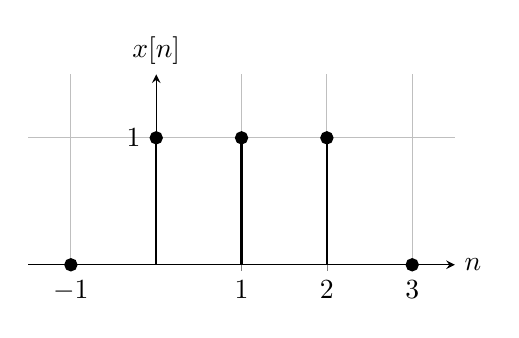
\begin{tikzpicture}
    \begin{axis}[
        width=7cm,
        height=4cm,
        axis lines=middle,
        xmin=-1.5, xmax=3.5,
        ymin=0, ymax=1.5,
        xtick={-1,0,1,2,3},
        ytick={0,1},
        xlabel={$n$},
        ylabel={$x[n]$},
        xlabel style={
            at={(axis description cs:1,0)},
            anchor=west
        },
        ylabel style={
            at={(axis description cs:0.3,1)},
            anchor=south,
            rotate=0
        },
        grid = both
    ]

    \addplot[
        ycomb,
        mark=*,
        thick
    ] coordinates {
        (-1,0)
        (0,1)
        (1,1)
        (2,1)
        (3,0)
    };

    \end{axis}
\end{tikzpicture}
\end{subfigure}
\hfill
\begin{subfigure}{0.48\textwidth}
\centering
\begin{tikzpicture}
    \begin{axis}[
        width=7cm,
        height=4cm,
        axis lines=middle,
        xmin=-0.5, xmax=3.5,
        ymin=0, ymax=1.5,
        xtick={0,1,2,3},
        ytick={0,1},
        xlabel={$n$},
        ylabel={$h[n]$},
        xlabel style={
            at={(axis description cs:1,0)},
            anchor=west
        },
        ylabel style={
            at={(axis description cs:0.15,1)},
            anchor=south,
            rotate=0
        },
        grid = both
    ]

    \addplot[
        ycomb,
        mark=*,
        thick
    ] coordinates {
        (0,0)
        (1,1)
        (2,1)
        (3,0)
    };

    \end{axis}
\end{tikzpicture}
\end{subfigure}
\caption{}
\label{fig:q4}
\end{figure}
\end{enumerate}

\end{document}
